\paragraph{Caso d'uso UC7.1.4:  Modifica Foto Utente}
\label{UC7_1_4}
\begin{figure}[ht]
	\centering
	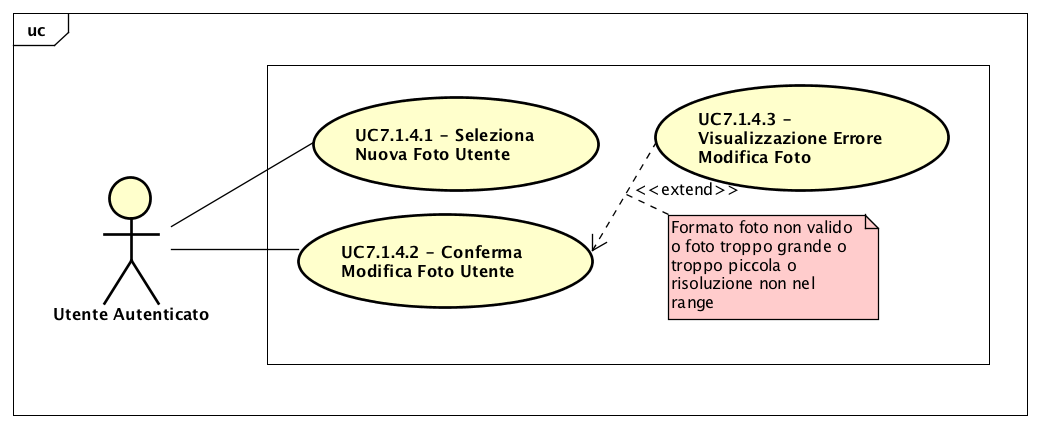
\includegraphics[scale=0.45]{UML/UC7_1_4.png}
	\caption{UC4: Login}
\end{figure}
\FloatBarrier
\begin{tabular}{ l | p{11cm}}
	\hline
	\rowcolor{Gray}
	 \multicolumn{2}{c}{UC7.1.4 - Modifica Foto Utente} \\
	 \hline
		\textbf{Attori} & Utente Autenticato \\
	\textbf{Descrizione} & Gli utenti possono modificare la propria Foto Profilo Utente selezionandola dal loro dispositivo\\
	\textbf{Pre-Condizioni} & L'utente e' nella schermata di gestione Profilo\\
	\textbf{Post-Condizioni} & L'utente ha modificato con successo la propria Foto Profilo \\
	\textbf{Scenario Principale} & 
	\begin{enumerate*}[label=(\arabic*.),itemjoin={\newline}]
		\item L'utente puo' inserire selezionare una Nuova Foto (UC7.1.4.1)
		\item L'utente conferma la modifica alla Foto Profilo (UC7.1.2.2)
	\end{enumerate*}\\
	\textbf{Scenari Alternativi} & 
	\begin{enumerate*}[label=(\arabic*.),itemjoin={\newline}]
		\item L'utente visualizza un errore nella modifica della Foto (UC7.1.2.3)
	\end{enumerate*}\\
\end{tabular}
